%----------------------------------------------------------------------------------------
%    PACKAGES AND THEMES
%----------------------------------------------------------------------------------------

\documentclass[aspectratio=169,xcolor=dvipsnames]{beamer}
\usetheme{SimpleDarkBlue}
\usepackage{tikz}
\usetikzlibrary{arrows.meta,decorations.pathmorphing,positioning}
\usepackage{graphicx}
\usepackage{pdfpages}
\usepackage{graphicx} % Allows including images
\usepackage{booktabs} % Allows the use of \toprule, \midrule and \bottomrule in tables
\usepackage{hyperref}
%----------------------------------------------------------------------------------------
%    TITLE PAGE
%----------------------------------------------------------------------------------------

\title{Improving Group Fairness in Knowledge Distillation
via Laplace Approximation of Early Exits}
% \subtitle{Experiments on Confidence Scoring}

\author{ Edvin 24V0074 \and Sagar 24D0367 }
% Kapil 210100079 }

\institute
{
    CS 769 \\
    Optimization in Machine Learning % Your institution for the title page
}
\date{2 May 2025} % Date, can be changed to a custom date

%----------------------------------------------------------------------------------------
%    PRESENTATION SLIDES
%----------------------------------------------------------------------------------------

\begin{document}

\begin{frame}
    % Print the title page as the first slide
    \titlepage
\end{frame}

\begin{frame}{Overview}
    % Throughout your presentation, if you choose to use \section{} and \subsection{} commands, these will automatically be printed on this slide as an overview of your presentation
    \tableofcontents
\end{frame}

\section{Recap from Seminar}

\begin{frame}{Recap from Seminar}
    \begin{itemize}
        \item<1-> Knowledge Distillation as an effective way to distill knowledge from teacher to student% 
        \item<2-> Teacher Provides "Soft Targets"
        \item<3-> Loss: kl divergence $+$ cross-entropy
        \item<4-> Student model relies on spurious correlations
        \item<5-> Student's early Layers overconfident on hard instances
        \item<6-> DEDIER loss
        \[ \mathcal{L}_{student} =
          \sum_{D_w}^{} (1- \lambda) \cdot l_{ce} 
          + \lambda \cdot \textbf{wt} \cdot l_{kd} \] 
          where \(\bf{wt} = \exp^{\beta.\bf{cm}.\alpha} \) and \(\bf{cm(p)} = p_{max} - \max_{p_k \in \bf{p} - p_{max}} p_k \) 
    \end{itemize}
\end{frame}

\begin{frame}{Recap from Seminar}
    \begin{itemize}
        \item<1-> Two alternate approaches for estimating uncertainity in prediction in early exit layers.
        \item<2-> \cite{meronen_fixing_2023} used Laplace approximation for bayesian posterior at exit layer.
        \item<3-> \cite{jazbec_early-exit_2024} used AVCS based on Predictive-likelihood ratio to get confidence intervals for predictions.
        \item<4-> Experiment: Laplace Approximation based uncertainity estimate to reweight both the losses.
    \end{itemize}
\end{frame}

\begin{frame}{Recap from Seminar}

    \only<1>{
        \begin{figure}
            \caption{}
            \centering
            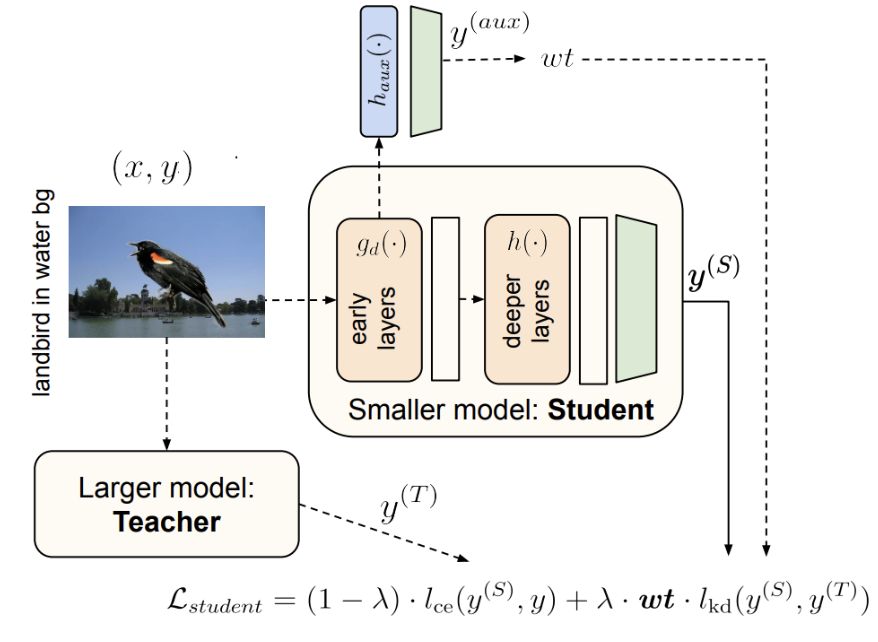
\includegraphics[width=0.6\textwidth]{figs/fig_4.png}
        \end{figure}
    }

    \only<2>{
        \begin{figure}
            \caption{}
            \centering
            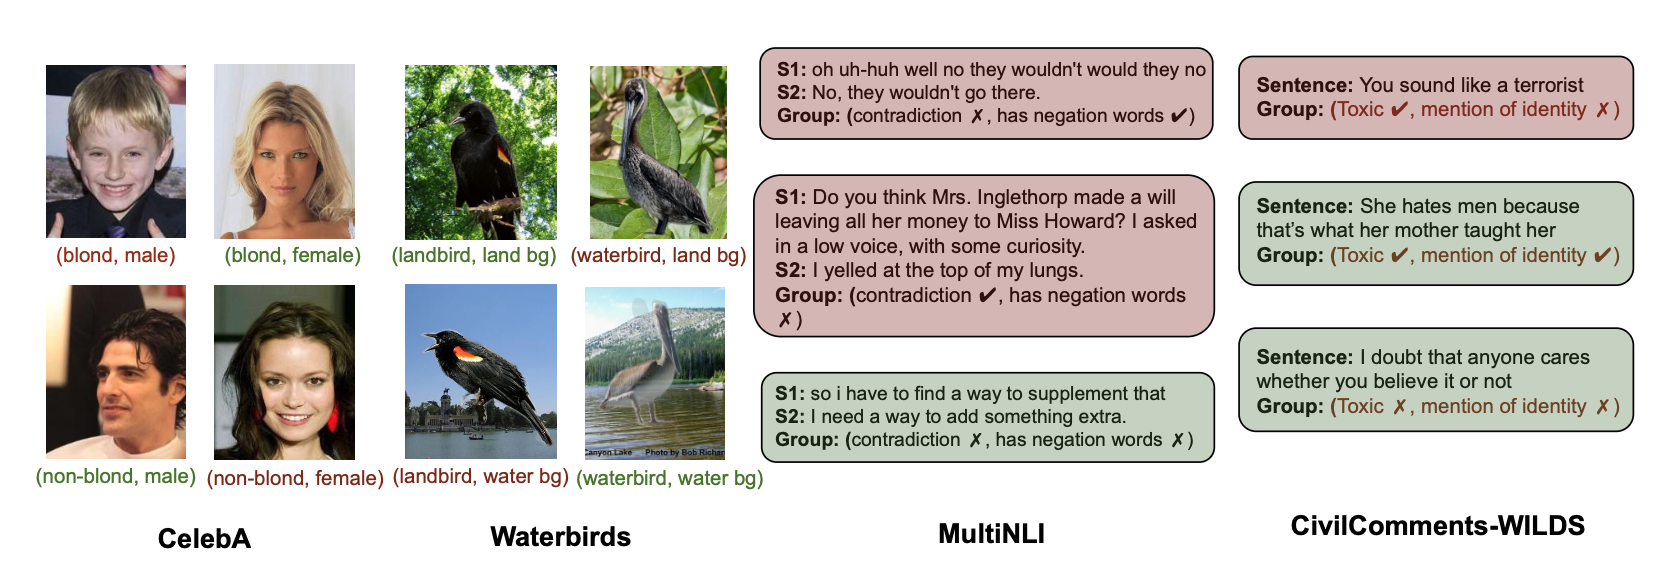
\includegraphics[width=\textwidth]{figs/fig_6.png}
        \end{figure}
    }

    \only<3>{
        \begin{figure}
            \caption{}
            \centering
            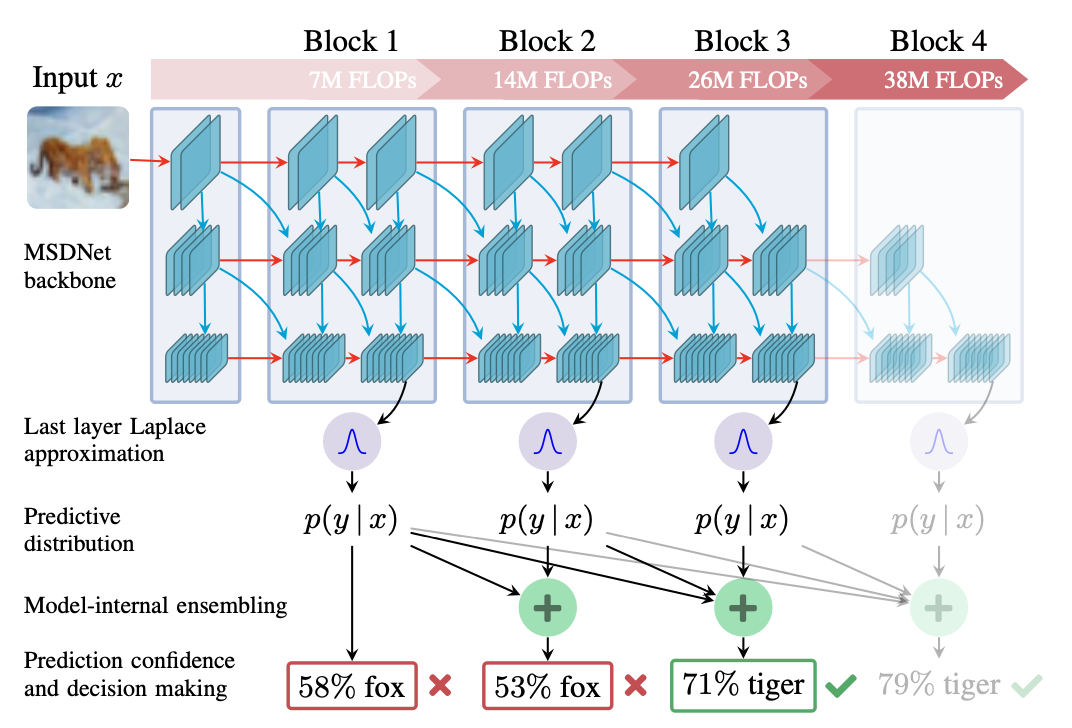
\includegraphics[width=0.4\linewidth]{figs/Screenshot 2025-04-08 at 15.02.28.png}
        \end{figure}
    }

    \only<4>{
        \begin{figure}
            \caption{}
            \centering
            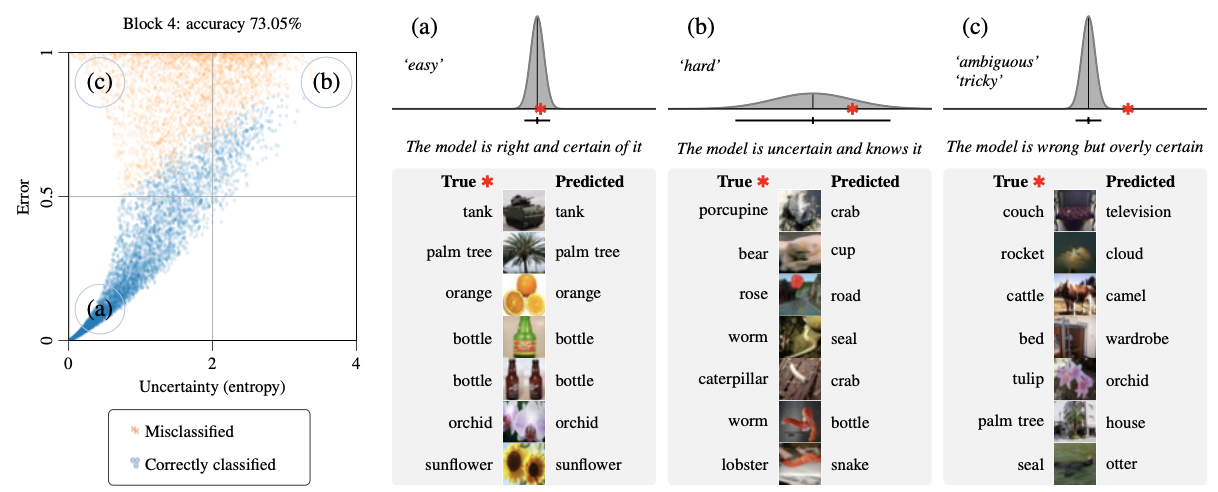
\includegraphics[width=0.7\linewidth]{figs/Screenshot 2025-04-08 at 15.14.46.png}
        \end{figure}
    }
\end{frame}

\begin{frame}{Recap from Seminar}
    \begin{itemize}
        \item<1-> Bayesian treatment of parameters
        \[
        p(\boldsymbol{\theta} \mid \mathcal{D}_{\text{train}})
        = \frac{p(\mathcal{D}_{\text{train}} \mid \boldsymbol{\theta}) \, p(\boldsymbol{\theta})}{\int_{\boldsymbol{\theta}} p(\mathcal{D}_{\text{train}}, \boldsymbol{\theta}) \, d\boldsymbol{\theta}}
        = \frac{\text{[likelihood]} \times \text{[prior]}}{\text{[model evidence]}}
    \]
        \item<2-> MAP estimate can be found by maximising the unnormalised posterior:
        \[
        \hat{\boldsymbol{\theta}} = \arg\max_{\boldsymbol{\theta}} \log p(\mathcal{D}_{\text{train}} \mid \boldsymbol{\theta}) + \log p(\boldsymbol{\theta})
              \]
        \item<3-> Gaussian distribution via laplace approximation
        \[
        p(\hat{\mathbf{z}}_i \mid \mathbf{x}_i) = \mathcal{N}(\hat{\mathbf{W}}_{\text{MAP}}^\top \hat{\boldsymbol{\phi}}_i, \, (\hat{\boldsymbol{\phi}}_i^\top \mathbf{V} \hat{\boldsymbol{\phi}}_i) \mathbf{U})
        \]
        \[
            \mathbf{V}^{-1} \otimes \mathbf{U}^{-1} = \mathbf{H}^{-1}
        \]
        \item<4-> Samples
        \[
         \hat{\mathbf{z}}_i^{(l)} = \hat{\mathbf{W}}_{\text{MAP}}^\top \hat{\boldsymbol{\phi}}_i + (\hat{\boldsymbol{\phi}}_i^\top \mathbf{V} \hat{\boldsymbol{\phi}}_i)^{\frac{1}{2}} (\mathbf{L} \mathbf{g}^{(l)})
        \]
        {\footnotesize \quad $\mathbf{g}^{(l)} \sim \mathcal{N}(0, \mathbf{I})$ and $\mathbf{L}$ is the Cholesky factor of $\mathbf{U}$}
    \end{itemize}
\end{frame}

\section{Experiments And Results}

\begin{frame}{Experiments And Results}

    \only<1>{
        \begin{\begin{itemize}
            \item The MultiNLI dataset \cite{williams2018broad} was used
        \end{itemize}
        }
    }

    \only<2>{
        \begin{figure}
            \caption{}
            \centering
            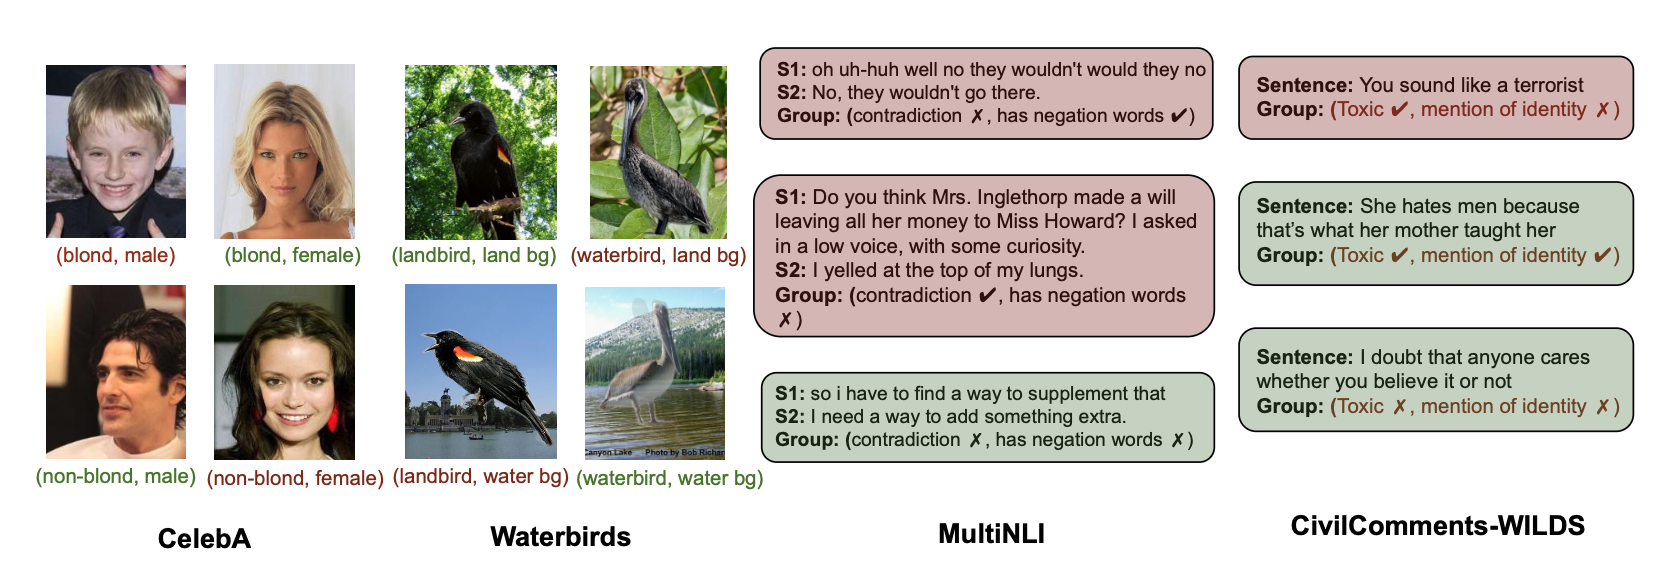
\includegraphics[width=\textwidth]{figs/fig_6.png}
        \end{figure}
    }

    \only<3>{
        \begin{figure}
            \caption{}
            \centering
            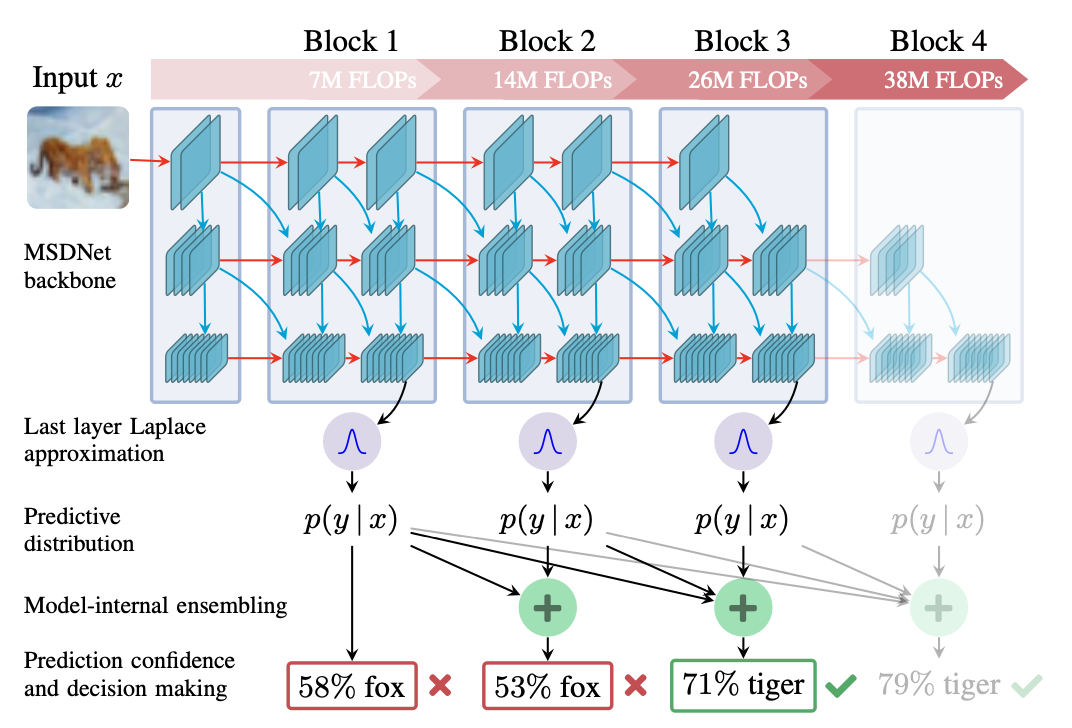
\includegraphics[width=0.4\linewidth]{figs/Screenshot 2025-04-08 at 15.02.28.png}
        \end{figure}
    }

    \only<4>{
        \begin{figure}
            \caption{}
            \centering
            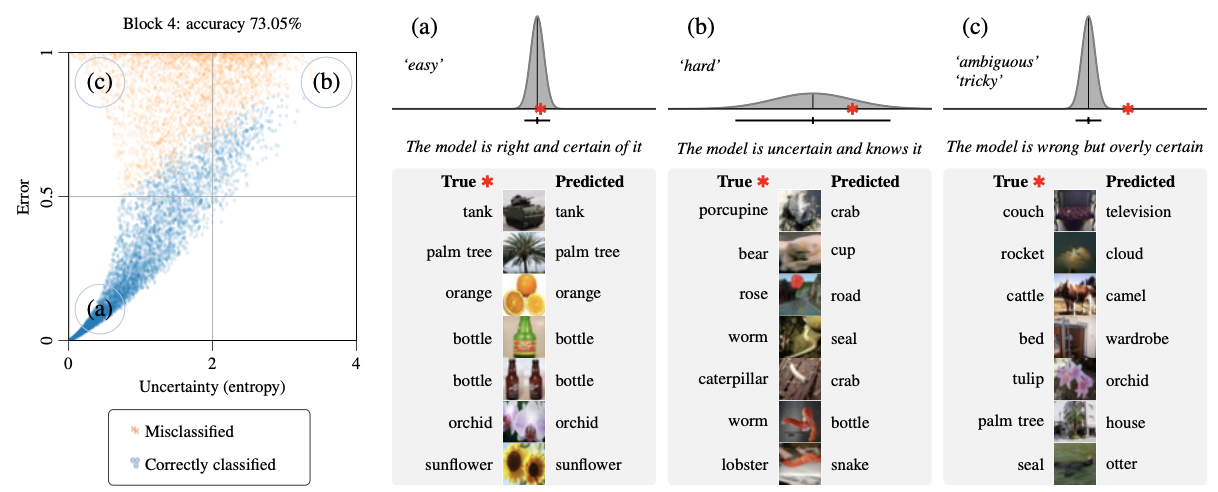
\includegraphics[width=0.7\linewidth]{figs/Screenshot 2025-04-08 at 15.14.46.png}
        \end{figure}
    }
\end{frame}

\section{Analysis And Future Work}




% \againframe<3-4>{slide:KD}
% \item<2-> Smaller Student model that mimics larger teacher model that generalises well
% \item<3-> The negative examples give info about dataset that is not captured by the cross entropy loss
% \item<4-> Teacher Provides "Soft Targets"
% \item<5-> minimise the kl divergence of last layer logits of the teacher along with cross entropy loss
% \begin{tikzpicture}<1>
%     \node at (0,0){Text Test};
% \end{tikzpicture}

\begin{frame}{References}
    \footnotesize
    %  \bibliography{reference.bib}
    \bibliographystyle{apalike}
    \bibliography{optML.bib}
\end{frame}

\end{document}
